\begin{figure*}[t]
	\centering
	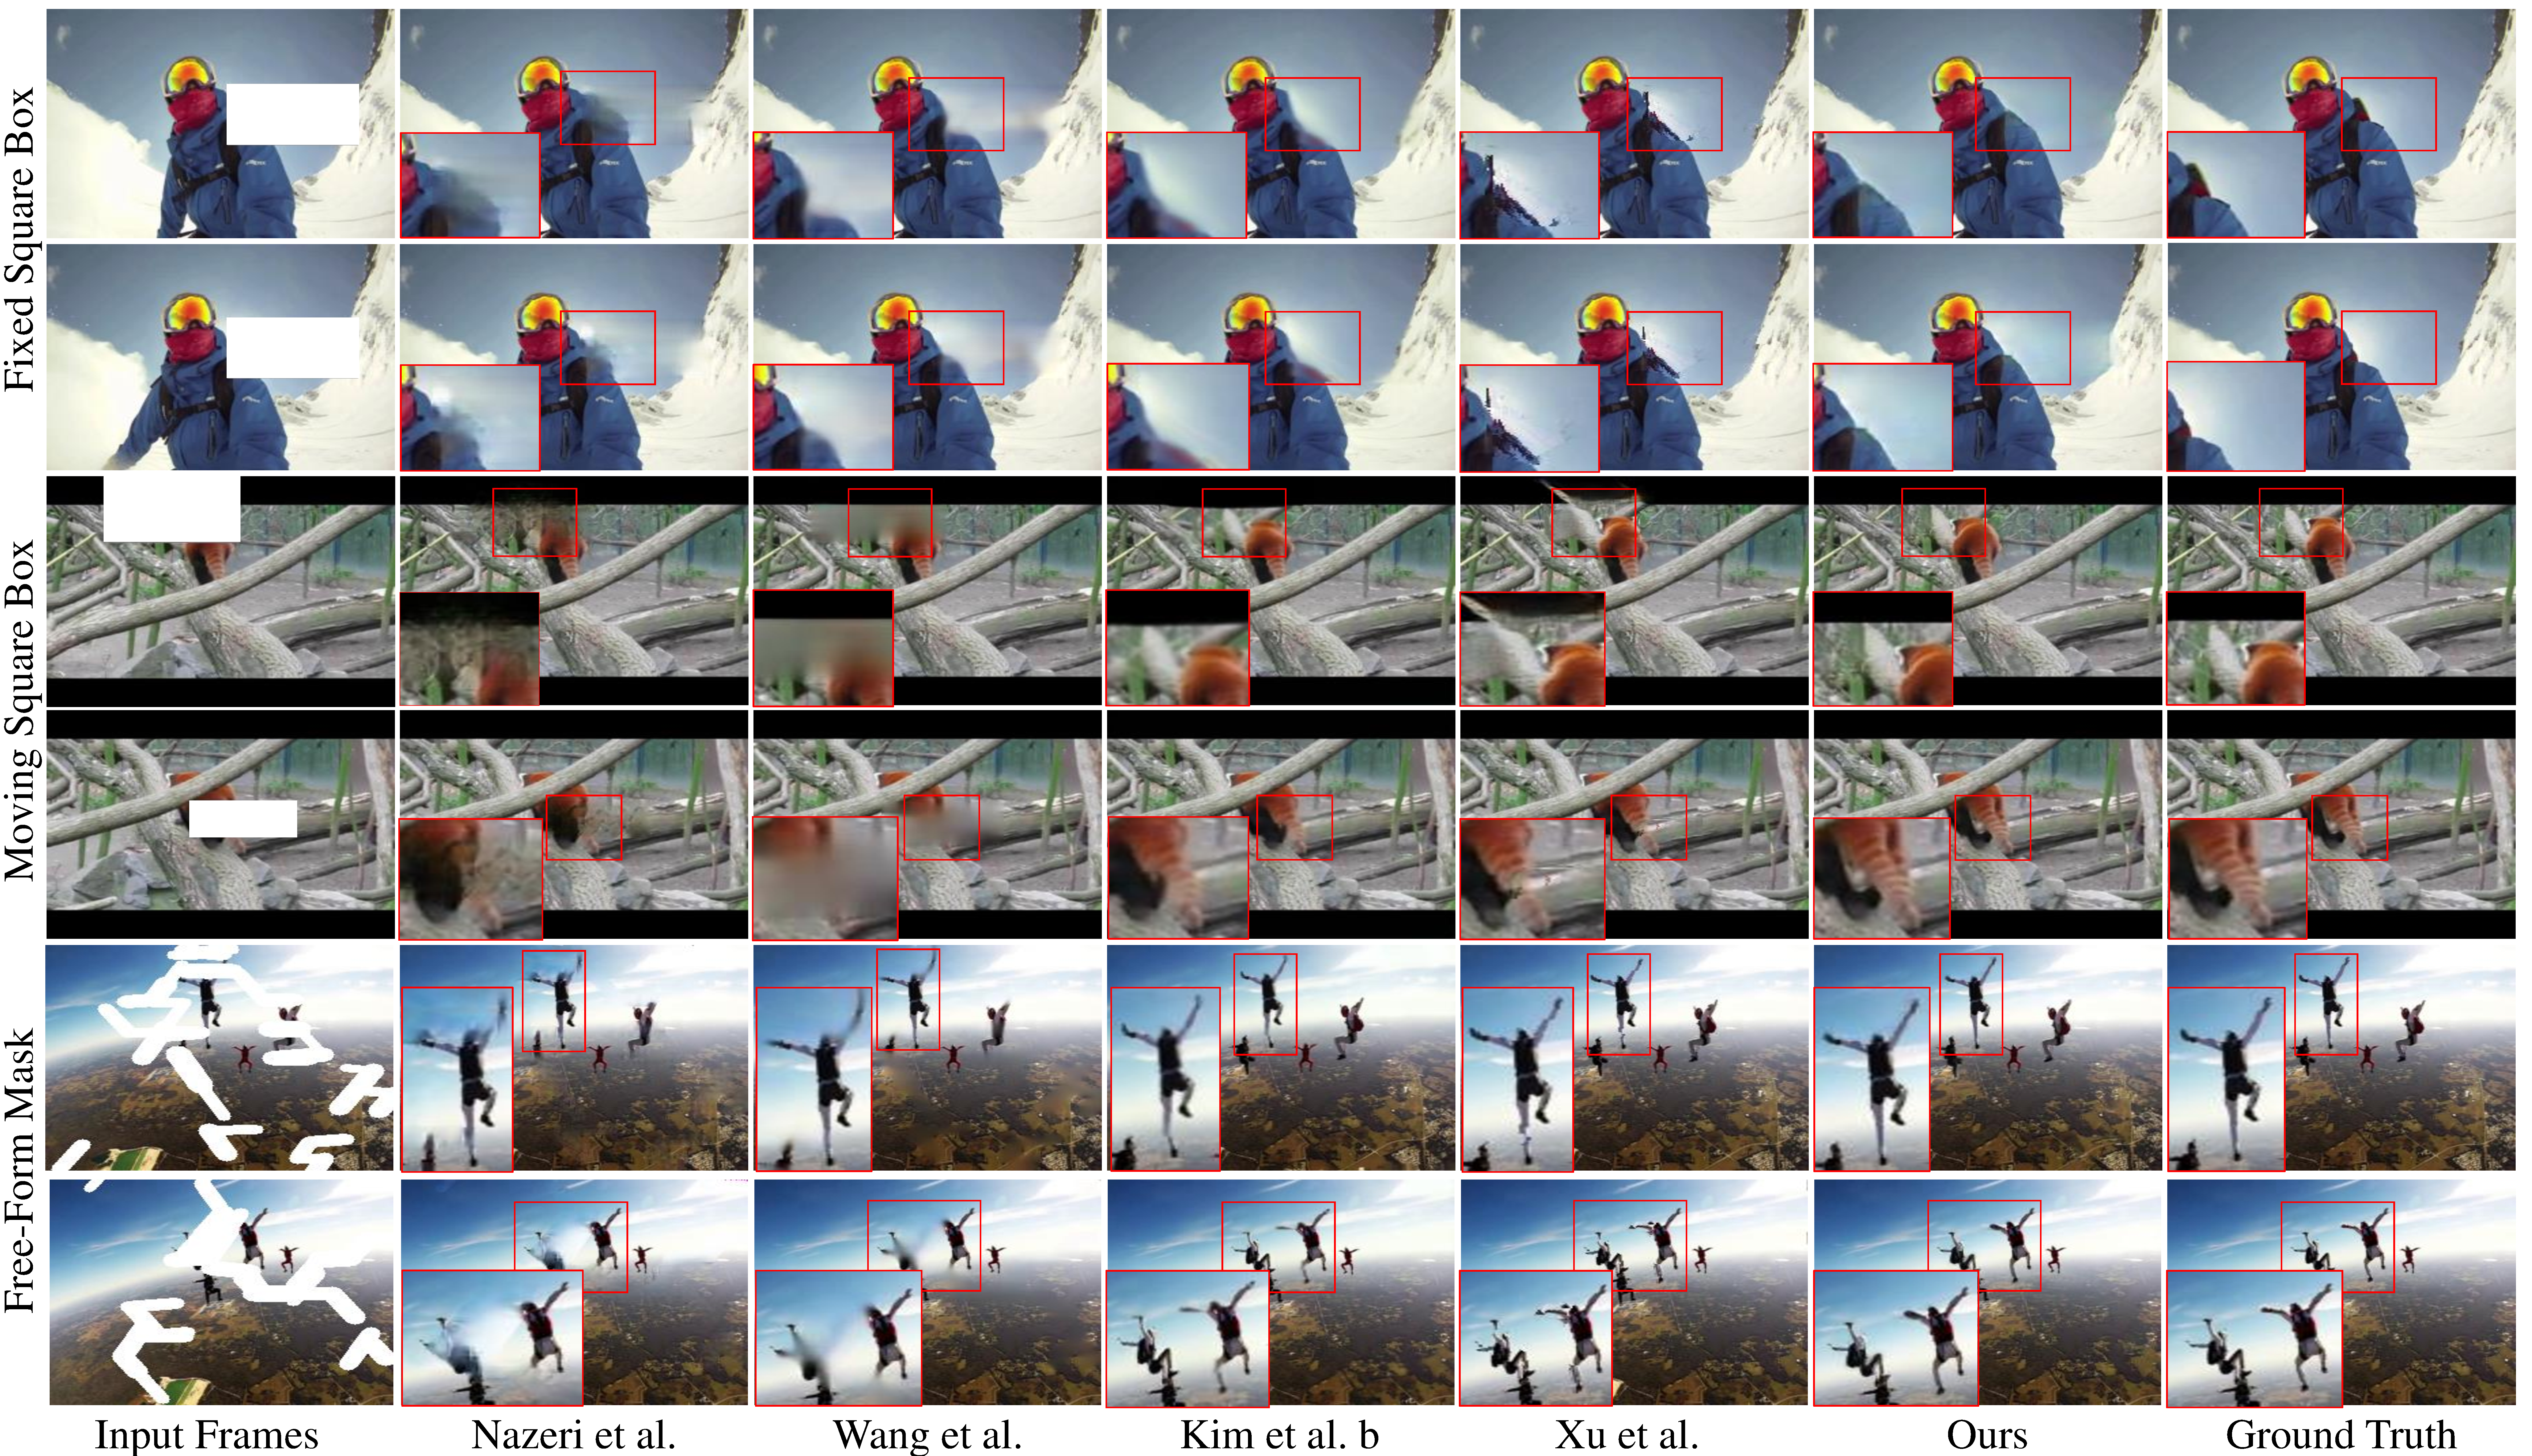
\includegraphics[width=1.5\columnwidth]{viszong} % Reduce the figure size so that it is slightly narrower than the column. Don't use precise values for figure width.This setup will avoid overfull boxes. 
	\caption{Visualization.}
	\label{viszong}
\end{figure*}


\section{Experiments}


\mdf{In order to evaluate the effect of different components in our STSTNet and compare with other state-of-the-art approaches, we conduct a series of experiments on two datasets...}
We test on two datasets, YoutubeVOS \cite{xu2018youtube} and DAVIS \cite{davis_2017}, to compare the proposed STSENet with state-of-the-art methods. %Several ablation studies are conducted to prove the effectiveness of spatial details and temporal information in video inpainting.
\subsection{Experimental Settings}
\textbf{Dataset.} 
\mdf{Two datasets, YoutubeVOS \cite{xu2018youtube} and DAVIS \cite{davis_2017} are widely used for evaluation in recent video inpainting approaches. }
\textbf{YoutubeVOS} is a large-scale dataset that contains 4,453 YouTube video clips. These videos are close to real-world scenario with 70+ common objects. 
The videos are split into three parts, 3,471 for training, 474 for validating, and 508 for testing. \cxj{randomly? or we use the same splitting set? }
\textbf{DAVIS} dataset contains 150 video clips, among which 90 are densely foreground annotated. \cxj{what do you mean here? The foreground objects are annotated? what does "densely" mean? what is the relationship with the annotation and our inpainting?}
The videos are complex with occlusions, fast motion, and various objects. 

\noindent \textbf{Mask Setting.} Considering various real-world applications, we test our method on four kinds of mask settings in this paper. 
They are different in shapes and positions of the missing regions.
\begin{enumerate}
	\item Fixed square mask. The size and position of the missing square region are fixed through the whole video. 
	\item Moving square mask. The position and size of the square mask change over frames. 
	\item Free-from mask. We apply irregular mask which imitates hand-drawn masks on each frame, following \cite{liu2018partialinpainting}. 
	\item Foreground object mask. This type of masks are defined to line out the foreground objects in videos.
\end{enumerate}

	
\noindent \textbf{Implementation Details.} 
In the data preparation stage, we random sample a clip \cxj{how long?} from each video in the datasets and resize the video frames into $256\times256$.
%
During training, we first train our ENet and FNet jointly using Adam optimizer with $\beta=(0.9, 0.999)$.
The learning rate is set to $1e-4$ for $N^E$ and $G^F$ and 1e-5 for $D^E$. Then, the STINet is trained with the learning rate of 1e-4 for $G^I$, and 4e-4 for $D^I$. We do not use weight decay in training.
As for the hyper-parameters, $\lambda_1=10.0,\lambda_2=\lambda_3=0.1,\lambda_4=300.0,\lambda_5=5.0$.

\noindent \textbf{Evaluation Metrics.} 
\mdf{We use three commonly-used metrics to quantitatively evaluate the performance of our method.} They are structural similarity index (SSIM) \cite{wang2004image}, peak signal-to-noise ratio (PSNR), and Fr{\'e}chet Inception Distance (FID) \cite{heusel2017gans}. 
\cxj{Where these three metrics are used compared with object removal?}
%
Besides, since there is no ground truth for the experiments of object removal, we conduct a user study for this mask setting. 


\subsection{Ablation Study}
To demonstrate the effectiveness of the proposed components in our STSENet, we first conduct an ablation study. 
We only use the first three mask settings on YoutubeVOS.
\cxj{for what reason? page limit of the paper? How about others? Can we result in the same conclusion for different mask settings?}

\noindent \textbf{Baselines.} Several variants of STSENet are defined as following. (1) STI w/o flow: The Spatio-Temporal Inpainting network without flow guidance \cxj{with or without EdgeNet and SEM?}. (2) STI w/o edge: The Spatio-Temporal Inpainting network without structure guidance. (3) STSENet w/o $\mathcal{L}_{fec}$: The Spatio-Temporal Inpainting network with guidance of both structure and motion, but $\mathcal{L}_{fec}$ is not used. (4) STSENet is the model which uses all modules proposed in this paper. 



\begin{figure}[t]
	\centering
	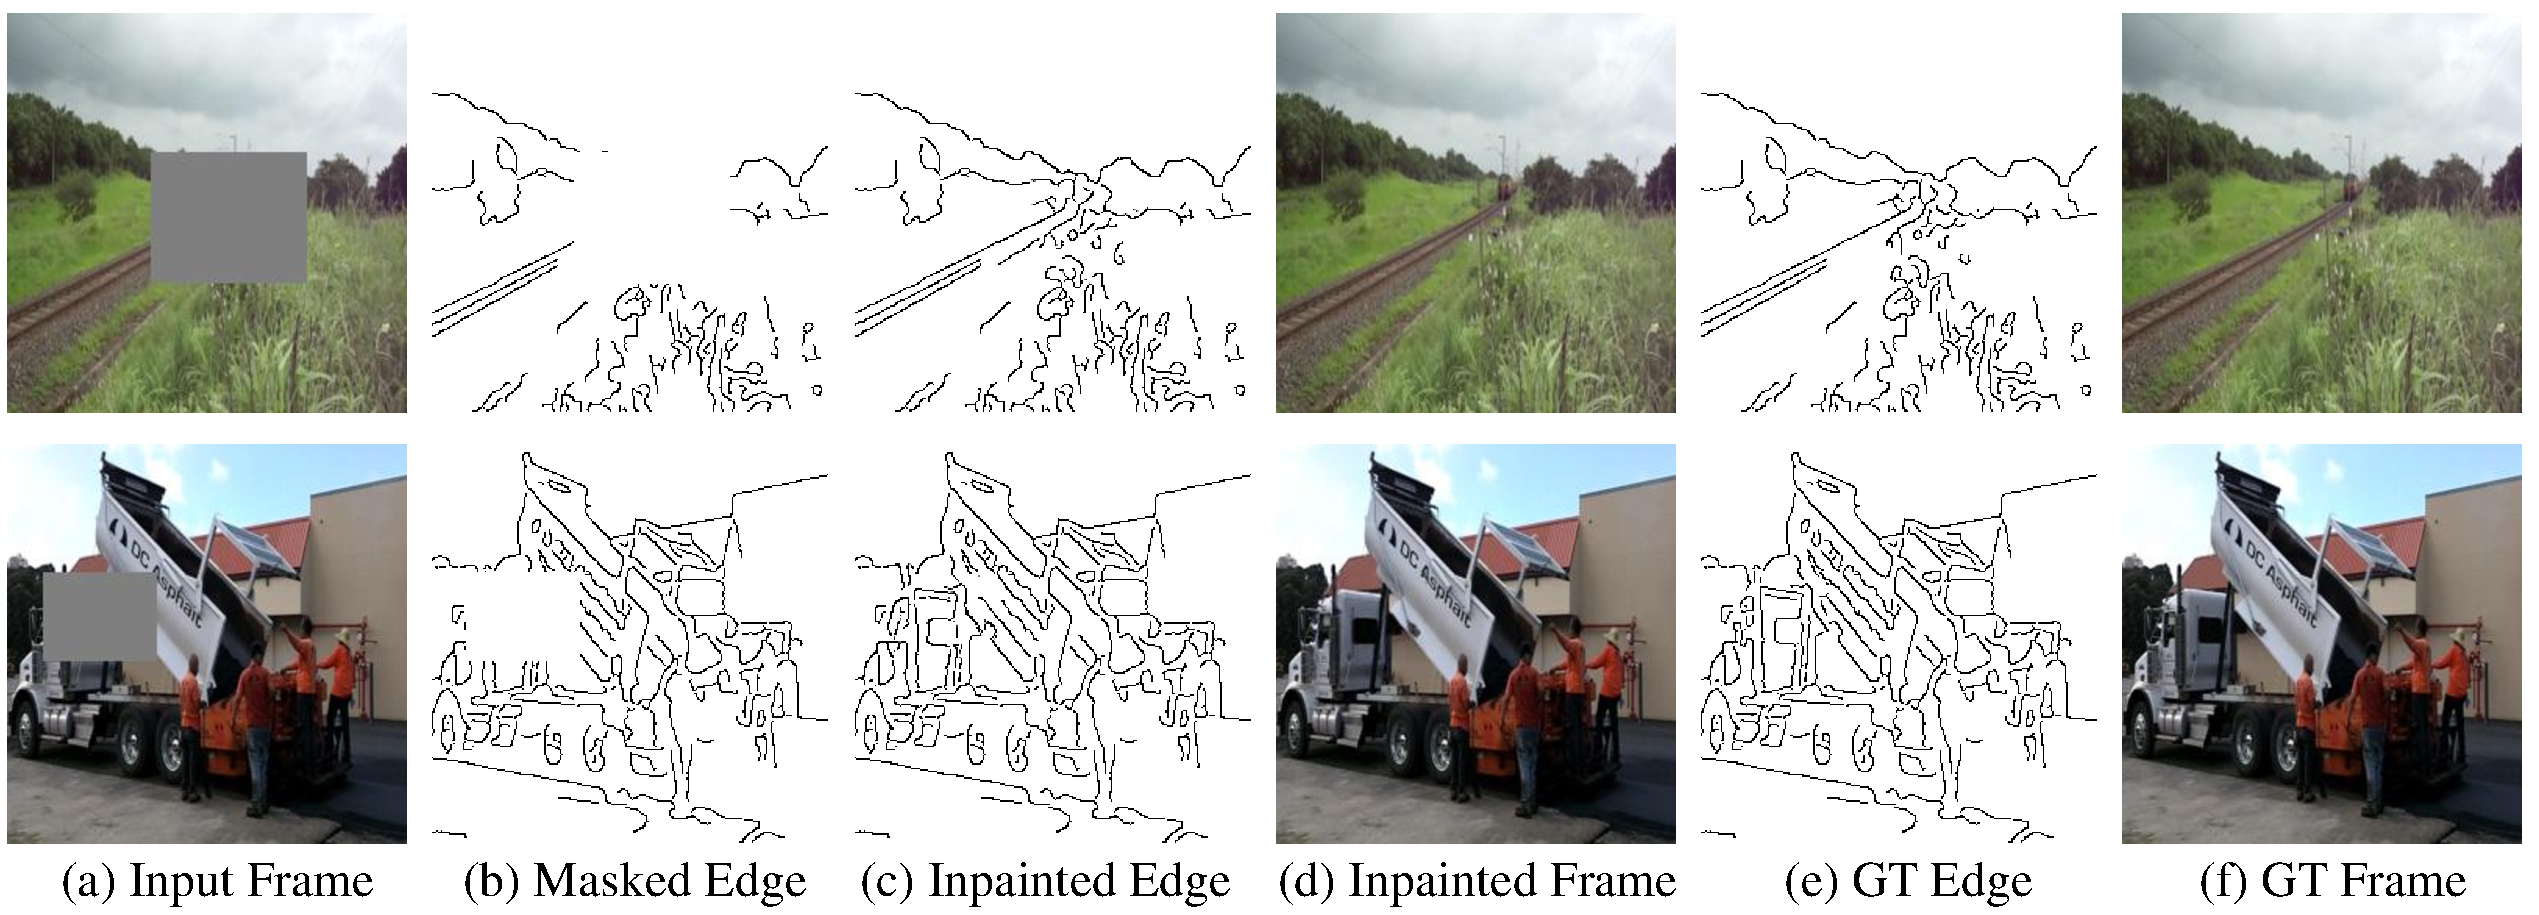
\includegraphics[width=1.0\columnwidth]{edgevis} % Reduce the figure size so that it is slightly narrower than the column. Don't use precise values for figure width.This setup will avoid overfull boxes. 
	\caption{Visualized effects of exploring structure edges in video inpainting.}
	\label{edgevis}
\end{figure}


\noindent \textbf{Effect of Structure Clues in STSENet.}
To evaluate the effects of structural information in video inpainting, we compare the performance of baselines in this part: STI and STI w/o SEM.
As shown in Table~\ref{tab:edge}, the network achieves better results when edge information is utilized,~\emph{i.e.} xxx improvements from STI w/o SEM to STI. It indicates that edge clues is an effective guidance in video inpainting, which helps the network to predict more accurate frames.
Furthermore, the superiority of SEM is evaluated by comparing its performance with the method, that replaces the attention map in Fig.~\ref{SEM} with edge map.
The results are reported in Table~\ref{tab:sem}, where SEM outperforms the simple edge attention over xxx.
This tells that the SEM can explore and encode the useful structure information into STI for structure-preserved video inpainting.

The visualization results are given in Fig.~\ref{edgevis}.
After exploring the edge structure, the inpainted frames become obviously better, with sharper object contours.
Thus, it is crucial to explore spatial details when inpainting the videos.
These results also show the strong edge inpainting ability of ENet.

\begin{table}[t]
	\caption{The effect of structure clues and temporal smoothening in STSENet. The mask number denotes the indexes of mask setting in the section Experimental Settings. We compare STI,STI w/o SEM, and  in three aspects of metrics.}\smallskip
	\centering
	\resizebox{.95\columnwidth}{!}{
		\smallskip\begin{tabular}{c|c|c|c|c}
			\hline
			Mask &Method  & PSNR & SSIM & FID\\
			\hline
			\multirow{3}*{Fixed}&STI &  &  & \\
			\cline{2-5} 
			&  STI w/o edge   &  &  & \\
			\cline{2-5} 
			&  STI w/o flow  &  &  & \\
			\hline
			
			\multirow{3}*{Moved}&STI &  &  & \\
			\cline{2-5} 
			&  STI w/o edge   &  &  & \\
			\cline{2-5} 
			&  STI w/o flow   &  &  & \\
			\hline
			\multirow{3}*{Free}&STI &  &  & \\
			\cline{2-5} 
			&  STI w/o edge   &  &  & \\
			\cline{2-5} 
			&  STI w/o flow   &  &  & \\
			\hline
		\end{tabular}
	}
	\label{tab:edge}
\end{table}
%We test baselines, 

\begin{table}[t]
	\caption{The effect of structure clues and temporal smoothening in STSENet. The mask number denotes the indexes of mask setting in the section Experimental Settings. We compare STI,STI w/o SEM, and  in three aspects of metrics.}\smallskip
	\centering
	\resizebox{.95\columnwidth}{!}{
		\smallskip\begin{tabular}{c|c|c|c|c}
			\hline
			Mask &Method  & PSNR & SSIM & FID\\
			\hline
			\multirow{2}*{Fixed}&STI+ edge attention &  &  & \\
			\cline{2-5} 
			&  STI + SEM   &  &  & \\
			\hline
		\end{tabular}
	}
	\label{tab:sem}
\end{table}

\noindent \textbf{Effect of Temporal Smoothening in STSENet.}
Temporal Consistency is an important factor in video inpainting. In STSENet, we utilize a flow warping loss to smoothen the artificial flickers and propagate complementary information from neighboring frames. 
Before temporal smoothing analysis, Fig.~\ref{flowvis} gives some results, which proves that FNet can effectively complete the missing flows.
To evaluate the impact of temporal smoothening in STI, we compare two baselines, STI and STI w/o flow.
As shown in Table~\ref{tab:edge}, STI works better than STI w/o flow, values...!!!.
The visualized results are shown in Fig.~\ref{}.
It can be observed that the Flickers are alleviated when motion guidance is involved. 
Both the quantitative and qualitative results prove that the motion information is beneficial to temporal consistency..

\begin{figure}[t]
	\centering
	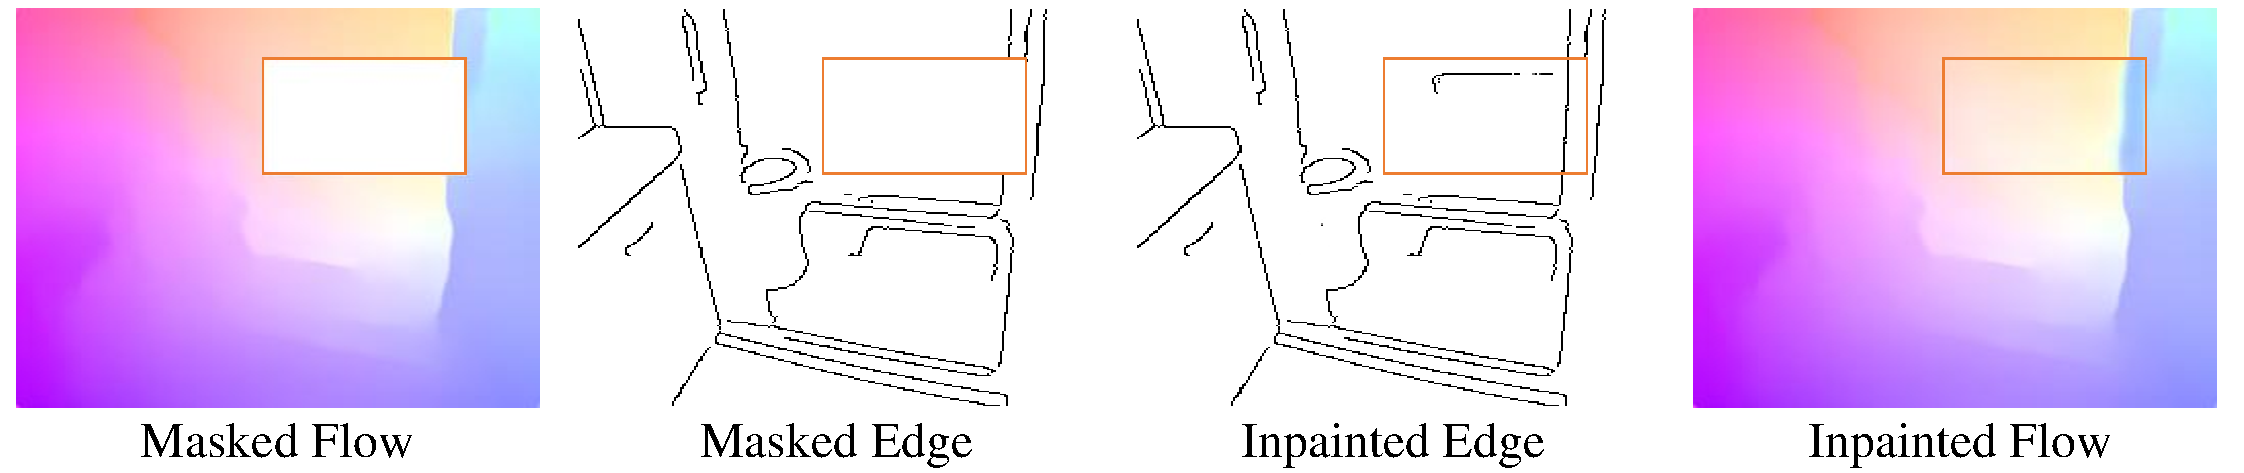
\includegraphics[width=1.0\columnwidth]{flowvis} % Reduce the figure size so that it is slightly narrower than the column. Don't use precise values for figure width.This setup will avoid overfull boxes. 
	\caption{Visualization.}
	\label{flowvis}
\end{figure}

\noindent \textbf{Effect of Flow-Edge Consistency Loss.}
Flow-edge consistency loss $\mathcal{L}_{fec}$ is designed for mutual improvement of optical flow and edge maps.
To demonstrate the effectiveness of $\mathcal{L}_{fec}$ in training, we compare the performances between STSENet w/o $\mathcal{L}_{fec}$ and STSENet. We use standard end-point-error (EPE) metric to evaluate the completion of optical flow. Besides, the well-completed flow and edge aid the final inpainting results, so the quality of final inpainting results also reflects the impact of $\mathcal{L}_{fec}$.
The quantitative results are shown in Table~\ref{tab:lfec}. It indicates that $\mathcal{L}_{fec}$ plays a positive role in prediction of flow and edge, which is helpful for video inpainting. The visulization results in Fig.~\ref{flowvis} shows that $\mathcal{L}_{fec}$ encourages the network to predict more accurate optical flow along the boundaries, which demonstrates the mutual improvement between flow and edge maps.
\begin{table}[t]
	\caption{The Impact of Flow-Edge Consistency Loss.}\smallskip
	
	\centering
	\resizebox{.95\columnwidth}{!}{
		\smallskip\begin{tabular}{c|c|c|c|c|c}
			\hline
			\multirow{2}*{Mask}& \multirow{2}*{Method} &Flow Completion & \multicolumn{3}{c}{Video Inpainting}\\
			\cline{3-6} 
			& &EPE & PSNR & SSIM & FID\\
			\hline
			\multirow{2}*{1}&STSENet w/o $\mathcal{L}_{fec}$&  &  & \\
			\cline{2-6} 
			&  STSENet     &  &  & \\
			\hline
			
			\multirow{2}*{2}&STSENet w/o $\mathcal{L}_{fec}$&  &  & \\
			\cline{2-6} 
			&  STSENet    &  &  & \\
			
			\hline
			\multirow{2}*{3}&STSENet w/o $\mathcal{L}_{fec}$&  &  & \\
			\cline{2-6} 
			&  STSENet   &  &  & \\
			\hline
		\end{tabular}
	}
	\label{tab:lfec}
\end{table}




\subsection{Comparisons with Existing Methods}
We compare our results with state-of-the-art inpainting methods \cite{nazeri2019edgeconnect,wang2019video,Xu_2019_CVPR,Kim_2019_CVPR1}. 
As shown in Table~\ref{tab:com}, STSENet achieves better results than other methods, which demonstrates the effectiveness of utilizing structural edges and optical flow in video inpainting.
We also give qualitative results in Fig.~\ref{viszong}. Compared with existing methods, inpainting results predicted by STSENet is more realistic with finer details and more temporal consistency.
\begin{table}[t]
	\caption{Comparisons with existing methods.}\smallskip
	
	\centering
	\resizebox{.95\columnwidth}{!}{
		\smallskip\begin{tabular}{c|c|c|c|c }
			\hline
			Mask &Method  & PSNR & SSIM & FID\\
			\hline
			\multirow{4}*{1}&\cite{nazeri2019edgeconnect} &  &  & \\
			\cline{2-5} 
			&  \cite{wang2019video}  &  &  & \\
			\cline{2-5} 
			&  \cite{Xu_2019_CVPR}  &  &  & \\
			\cline{2-5} 
			&  \cite{Kim_2019_CVPR1}  &  &  & \\
			\cline{2-5} 	
			&  STSENet  &  &  & \\
			\hline
			
			\multirow{4}*{2}&\cite{nazeri2019edgeconnect} &  &  & \\
			\cline{2-5} 
			&  \cite{wang2019video}  &  &  & \\
			\cline{2-5} 
			&  \cite{Xu_2019_CVPR}  &  &  & \\
			\cline{2-5} 
			&  \cite{Kim_2019_CVPR1}  &  &  & \\
			\cline{2-5} 	
			&  STSENet  &  &  & \\
			\hline
			
			\multirow{4}*{3}&\cite{nazeri2019edgeconnect} &  &  & \\
			\cline{2-5} 
			&  \cite{wang2019video}  &  &  & \\
			\cline{2-5} 
			&  \cite{Xu_2019_CVPR}  &  &  & \\
			\cline{2-5} 
			&  \cite{Kim_2019_CVPR1}  &  &  & \\
			\cline{2-5} 	
			&  STSENet  &  &  & \\
			\hline
			
		
		\end{tabular}
	}
	\label{tab:com}
\end{table}

\subsection{User Study}
Evaluation metrics can not fully reflect the quality of inpainted videos. So in addition to qualitative comparison, we also conduct a user study to evaluate our method. To


\section{Conclusion}
In this paper, we propose a novel video inpainting network called Spatio-Temporal Structure Enhancement Network (STSENet), which utilizes sturcture information and temproal clues to enhance spatio-temporal consistency. Specifically, we jointly complete edge maps and optical flow with a consistency loss, which helps to obtain temporal consistent edge and edge-clear optical flow. Then with the guidance of spatial details and motion tendency, spatio-temporal inpainting network is designed to predict the final video with fine spatial details few artificial flickers.
The state-of-the-art performance on both YouTube-VOS and DAVIS prove the effectiveness of exploring structural clues and optical flow in video inpainting.
 
